\subsection{\label{sec:level2}Two x-points}
For understanding the N-S-E-W convention of the secondary x-point, it is useful to consider the partition of the domain induced by any given separatrix. With these distinct regions in mind, we define N for the secondary x-point to be the in the direction of the region that contains the primary separatrix. We assign a Point object for this N direction some $\varepsilon$ distance away from the secondary x-point. The remaining secondary x-point directions (S, E, W, SE, SW, NE, NW) are obtained by the appropriate rotations of the established N Point.\\ \indent
This secondary x-point N-S-E-W criteria is not only a critical step for identification of a divertor configuration, but also provides a general plate naming scheme for all magnetic topologies. Just like the primary x-point case, we have the ``SW" and ``SE" directions of the secondary x-point intersect individual target plates. We can see this idea and the ideas discussed earlier in figure \ref{fig:xpt_2_directions}. To remain consistent with the primary x-point target plate naming scheme, we refer to these plates as ``plate\_W2" and ``plate\_E2" for the ``SW" and ``SE" directions respectively. The ``2" here indicates that these plates are unique to the cases with two x-points.
\begin{figure}[H]
    \centering
    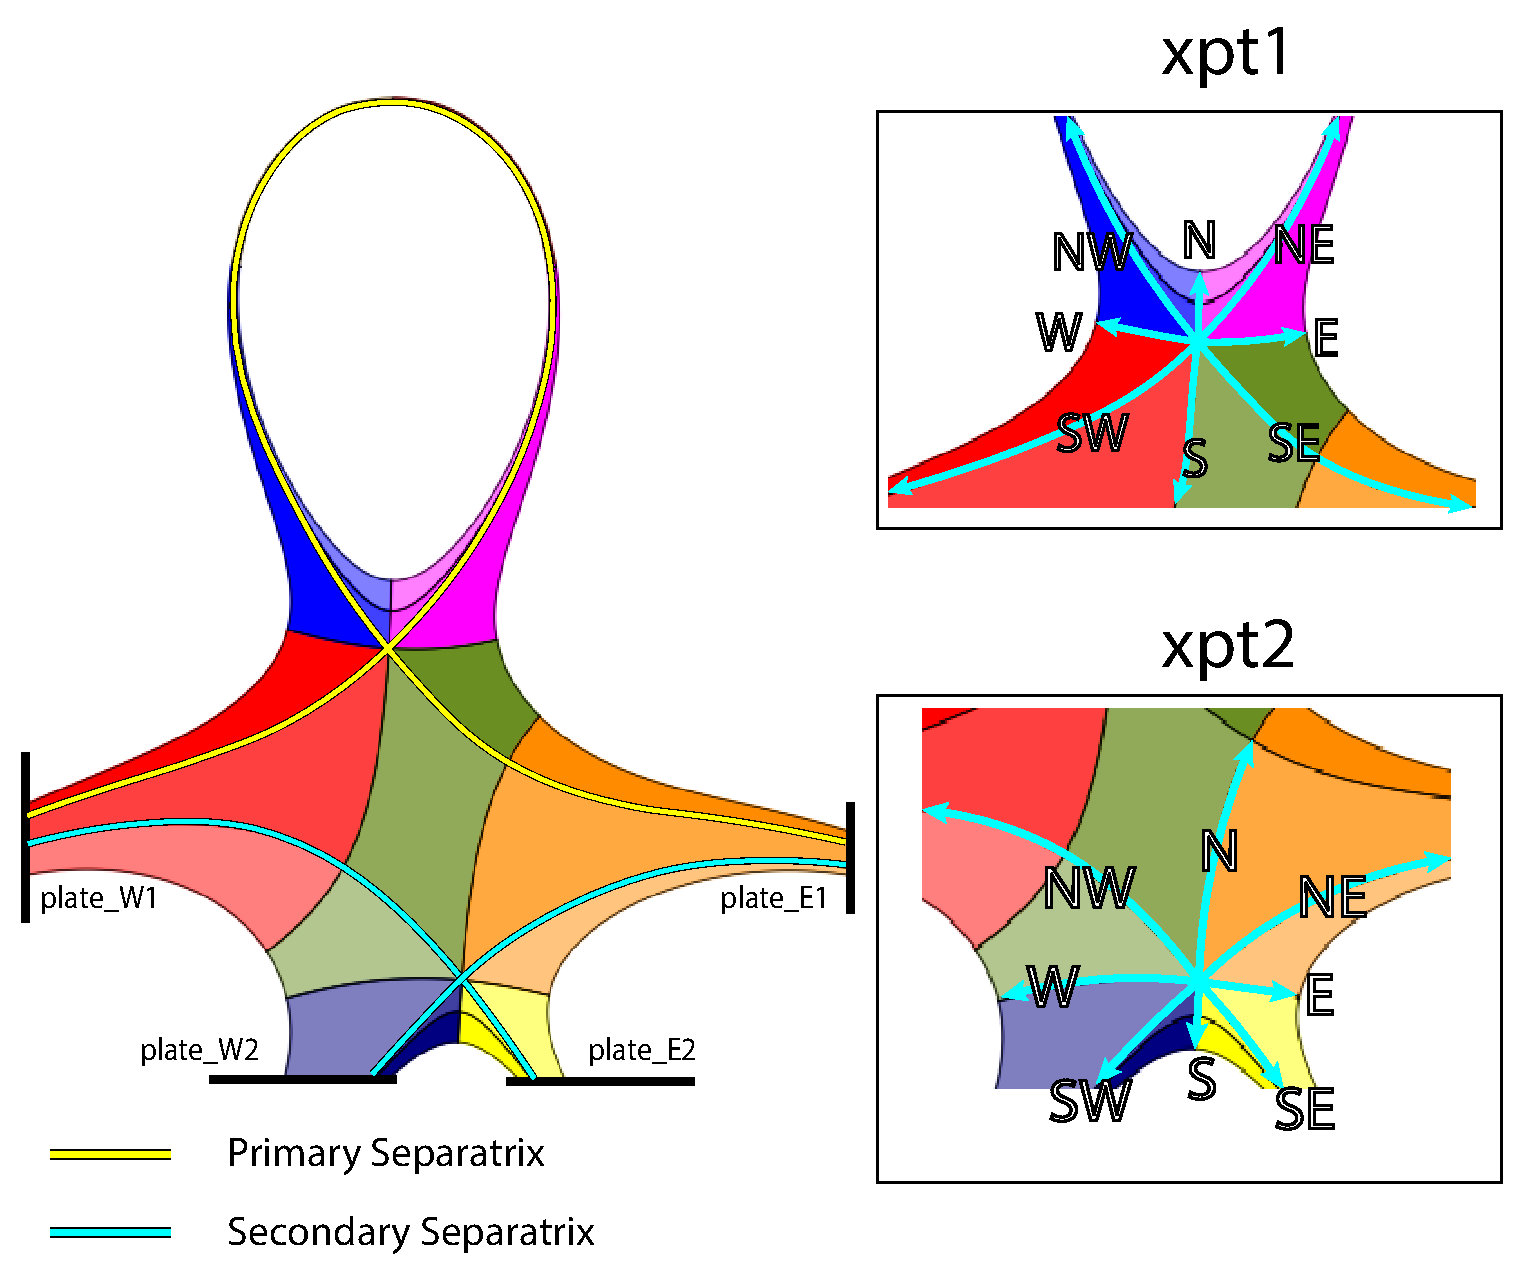
\includegraphics[width=\linewidth]{figures/xpt_2_directions.pdf}
    \caption{An SF75 divertor configuration illustrating the primary x-point and secondary x-point N-S-E-W labeling convention.}
    \label{fig:xpt_2_directions}
\end{figure}